
Per una corrente incomprimibile, $\bm{\nabla} \cdot \bm{u} = 0$, il campo di velocità può essere scritto come il rotore di un campo vettoriale $\bm{\psi}$, definito come \textit{potenziale vettore}\footnote{Un campo vettoriale $\bm{u} = \bm{\nabla} \times \bm{\psi}$ soddisfa identicamente la relazione $\bm{\nabla} \cdot \bm{u} = 0$, poichè la divergenza di un rotore è identicamente nulla,
\begin{equation}
  \bm{\nabla} \cdot \left( \bm{\nabla} \times \bm{\psi} \right) \equiv 0 \ .
\end{equation} }
\begin{equation}\label{eqn:psi}
 \bm{u} = \bm{\nabla} \times \bm{\psi} \ .
\end{equation}
Sfruttando un sistema di coordinate cartesiane, si può esprimere un campo di velocità incomprimibile bidimensionale $\bm{u}(x,y) = u_x(x,y) \bm{\hat{x}} + u_y(x,y) \bm{\hat{y}}$ utilizzando una funzione scalare $\psi(x,y)$, definita \textit{funzione di corrente}, come
\begin{equation}
\begin{cases}
 u_x & = \p{\psi}{y} \vspace{0.2cm} \\
 u_y & =-\p{\psi}{x} \ . \\
\end{cases}
\end{equation}
Con un calcolo diretto della divergenza, si può verificare che questo campo di velocità soddisfa il vincolo di incomprimibilità,
\begin{equation}
 \bm{\nabla} \cdot \bm{u} = \p{u_x}{x} + \p{u_y}{y} =
  \frac{\partial^2 \psi}{\partial x \partial y} - 
  \frac{\partial^2 \psi}{\partial y \partial x} = 0 \ ,
\end{equation}
sotto le ipotesi, soddisfatte per ``funzioni sufficientemente regolari'', del \textit{teorema di Schwarz}, che afferma l'uguaglianza delle derivate miste.

\vspace{0.2cm}
\'E possibile dimostrare che le isolinee della funzione $\psi(x,y)$, quelle curve sulle quali la funzione è costante, coincidono con le linee di corrente del campo di velocità.

\noindent
Le isolinee di una funzione sono perpendicolari al gradiente della funzione stessa.\footnote{
 Il gradiente $\bm{\nabla} f$ di una funzione $f$ è diretto lungo la direzione locale di massima crescita della funzione. La derivata direzionale della funzione $f$ nella direzione indicata dal versore $\bm{\hat{v}}$ è uguale a $\bm{\hat{v}} \cdot \bm{\nabla}f$. Lungo le isolinee di una funzione, la funzione è costante e quindi la sua derivata direzionale lungo quella direzione è nulla. Indicando con $\bm{\hat{t}}$ il versore tangente alle isolinee, si può quindi scrivere $\bm{\hat{t}} \cdot \bm{\nabla} f = 0$.
}
Se riusciamo a dimostrare che le linee di corrente (che sono definite come le curve parallele al campo di velocità) sono localmente perpendicolari al gradiente della funzione $\psi$, dimostriamo che queste sono localmente parallele (e quindi sono la stessa curva) alle isolinee di $\psi$ in uno spazio bidimensionale.

\noindent
Per dimostrare che le linee di corrente sono perpendicolari al gradiente di $\psi$, è sufficiente calcolare il prodotto scalare tra il campo di velocità e il gradiente di $\psi$,
\begin{equation}
 \bm{u} \cdot \bm{\nabla} \psi = u_x \, \p{\psi}{x} + u_y \, \p{\psi}{y}   
                               = \p{\psi}{y} \, \p{\psi}{x} + \left(-\p{\psi}{x} \right) \, \p{\psi}{y} = 0 \ .
\end{equation}
Nella relazione non sono stati indicati esplicitamente gli argomenti delle funzioni, che identificano un punto nello spazio. La relazione $\bm{u} \cdot \bm{\nabla} \psi = 0$ vale in ogni punto dello spazio e ci dice che il gradiente della funzione di corrente è perpendicolare al vettore velocità in ogni punto del dominio, come mostrato in figura \ref{fig:streaml}.

\begin{figure}[h!]
\centering
 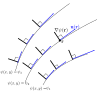
\includegraphics[width=0.75\textwidth]{./psi_streamlines}
 \caption{Relazione tra il campo e la funzione di corrente per un campo di velocità piano che soddisfa il vincolo di incomprimibilità. Il gradiente della funzione di corrente è perpendicolare in ogni punto al vettore velocità e, di conseguenza, le isolinee della funzione di corrente coincidono con le linee di corrente del campo di velocità.}\label{fig:streaml}
\end{figure}
